\documentclass[1p]{elsarticle_modified}
%\bibliographystyle{elsarticle-num}

%\usepackage[colorlinks]{hyperref}
%\usepackage{abbrmath_seonhwa} %\Abb, \Ascr, \Acal ,\Abf, \Afrak
\usepackage{amsfonts}
\usepackage{amssymb}
\usepackage{amsmath}
\usepackage{amsthm}
\usepackage{scalefnt}
\usepackage{amsbsy}
\usepackage{kotex}
\usepackage{caption}
\usepackage{subfig}
\usepackage{color}
\usepackage{graphicx}
\usepackage{xcolor} %% white, black, red, green, blue, cyan, magenta, yellow
\usepackage{float}
\usepackage{setspace}
\usepackage{hyperref}

\usepackage{tikz}
\usetikzlibrary{arrows}

\usepackage{multirow}
\usepackage{array} % fixed length table
\usepackage{hhline}

%%%%%%%%%%%%%%%%%%%%%
\makeatletter
\renewcommand*\env@matrix[1][\arraystretch]{%
	\edef\arraystretch{#1}%
	\hskip -\arraycolsep
	\let\@ifnextchar\new@ifnextchar
	\array{*\c@MaxMatrixCols c}}
\makeatother %https://tex.stackexchange.com/questions/14071/how-can-i-increase-the-line-spacing-in-a-matrix
%%%%%%%%%%%%%%%

\usepackage[normalem]{ulem}

\newcommand{\msout}[1]{\ifmmode\text{\sout{\ensuremath{#1}}}\else\sout{#1}\fi}
%SOURCE: \msout is \stkout macro in https://tex.stackexchange.com/questions/20609/strikeout-in-math-mode

\newcommand{\cancel}[1]{
	\ifmmode
	{\color{red}\msout{#1}}
	\else
	{\color{red}\sout{#1}}
	\fi
}

\newcommand{\add}[1]{
	{\color{blue}\uwave{#1}}
}

\newcommand{\replace}[2]{
	\ifmmode
	{\color{red}\msout{#1}}{\color{blue}\uwave{#2}}
	\else
	{\color{red}\sout{#1}}{\color{blue}\uwave{#2}}
	\fi
}

\newcommand{\Sol}{\mathcal{S}} %segment
\newcommand{\D}{D} %diagram
\newcommand{\A}{\mathcal{A}} %arc


%%%%%%%%%%%%%%%%%%%%%%%%%%%%%5 test

\def\sl{\operatorname{\textup{SL}}(2,\Cbb)}
\def\psl{\operatorname{\textup{PSL}}(2,\Cbb)}
\def\quan{\mkern 1mu \triangleright \mkern 1mu}

\theoremstyle{definition}
\newtheorem{thm}{Theorem}[section]
\newtheorem{prop}[thm]{Proposition}
\newtheorem{lem}[thm]{Lemma}
\newtheorem{ques}[thm]{Question}
\newtheorem{cor}[thm]{Corollary}
\newtheorem{defn}[thm]{Definition}
\newtheorem{exam}[thm]{Example}
\newtheorem{rmk}[thm]{Remark}
\newtheorem{alg}[thm]{Algorithm}

\newcommand{\I}{\sqrt{-1}}
\begin{document}

%\begin{frontmatter}
%
%\title{Boundary parabolic representations of knots up to 8 crossings}
%
%%% Group authors per affiliation:
%\author{Yunhi Cho} 
%\address{Department of Mathematics, University of Seoul, Seoul, Korea}
%\ead{yhcho@uos.ac.kr}
%
%
%\author{Seonhwa Kim} %\fnref{s_kim}}
%\address{Center for Geometry and Physics, Institute for Basic Science, Pohang, 37673, Korea}
%\ead{ryeona17@ibs.re.kr}
%
%\author{Hyuk Kim}
%\address{Department of Mathematical Sciences, Seoul National University, Seoul 08826, Korea}
%\ead{hyukkim@snu.ac.kr}
%
%\author{Seokbeom Yoon}
%\address{Department of Mathematical Sciences, Seoul National University, Seoul, 08826,  Korea}
%\ead{sbyoon15@snu.ac.kr}
%
%\begin{abstract}
%We find all boundary parabolic representation of knots up to 8 crossings.
%
%\end{abstract}
%\begin{keyword}
%    \MSC[2010] 57M25 
%\end{keyword}
%
%\end{frontmatter}

%\linenumbers
%\tableofcontents
%
\newcommand\colored[1]{\textcolor{white}{\rule[-0.35ex]{0.8em}{1.4ex}}\kern-0.8em\color{red} #1}%
%\newcommand\colored[1]{\textcolor{white}{ #1}\kern-2.17ex	\textcolor{white}{ #1}\kern-1.81ex	\textcolor{white}{ #1}\kern-2.15ex\color{red}#1	}

{\Large $\underline{12n_{0124}~(K12n_{0124})}$}

\setlength{\tabcolsep}{10pt}
\renewcommand{\arraystretch}{1.6}
\vspace{1cm}\begin{tabular}{m{100pt}>{\centering\arraybackslash}m{274pt}}
\multirow{5}{120pt}{
	\centering
	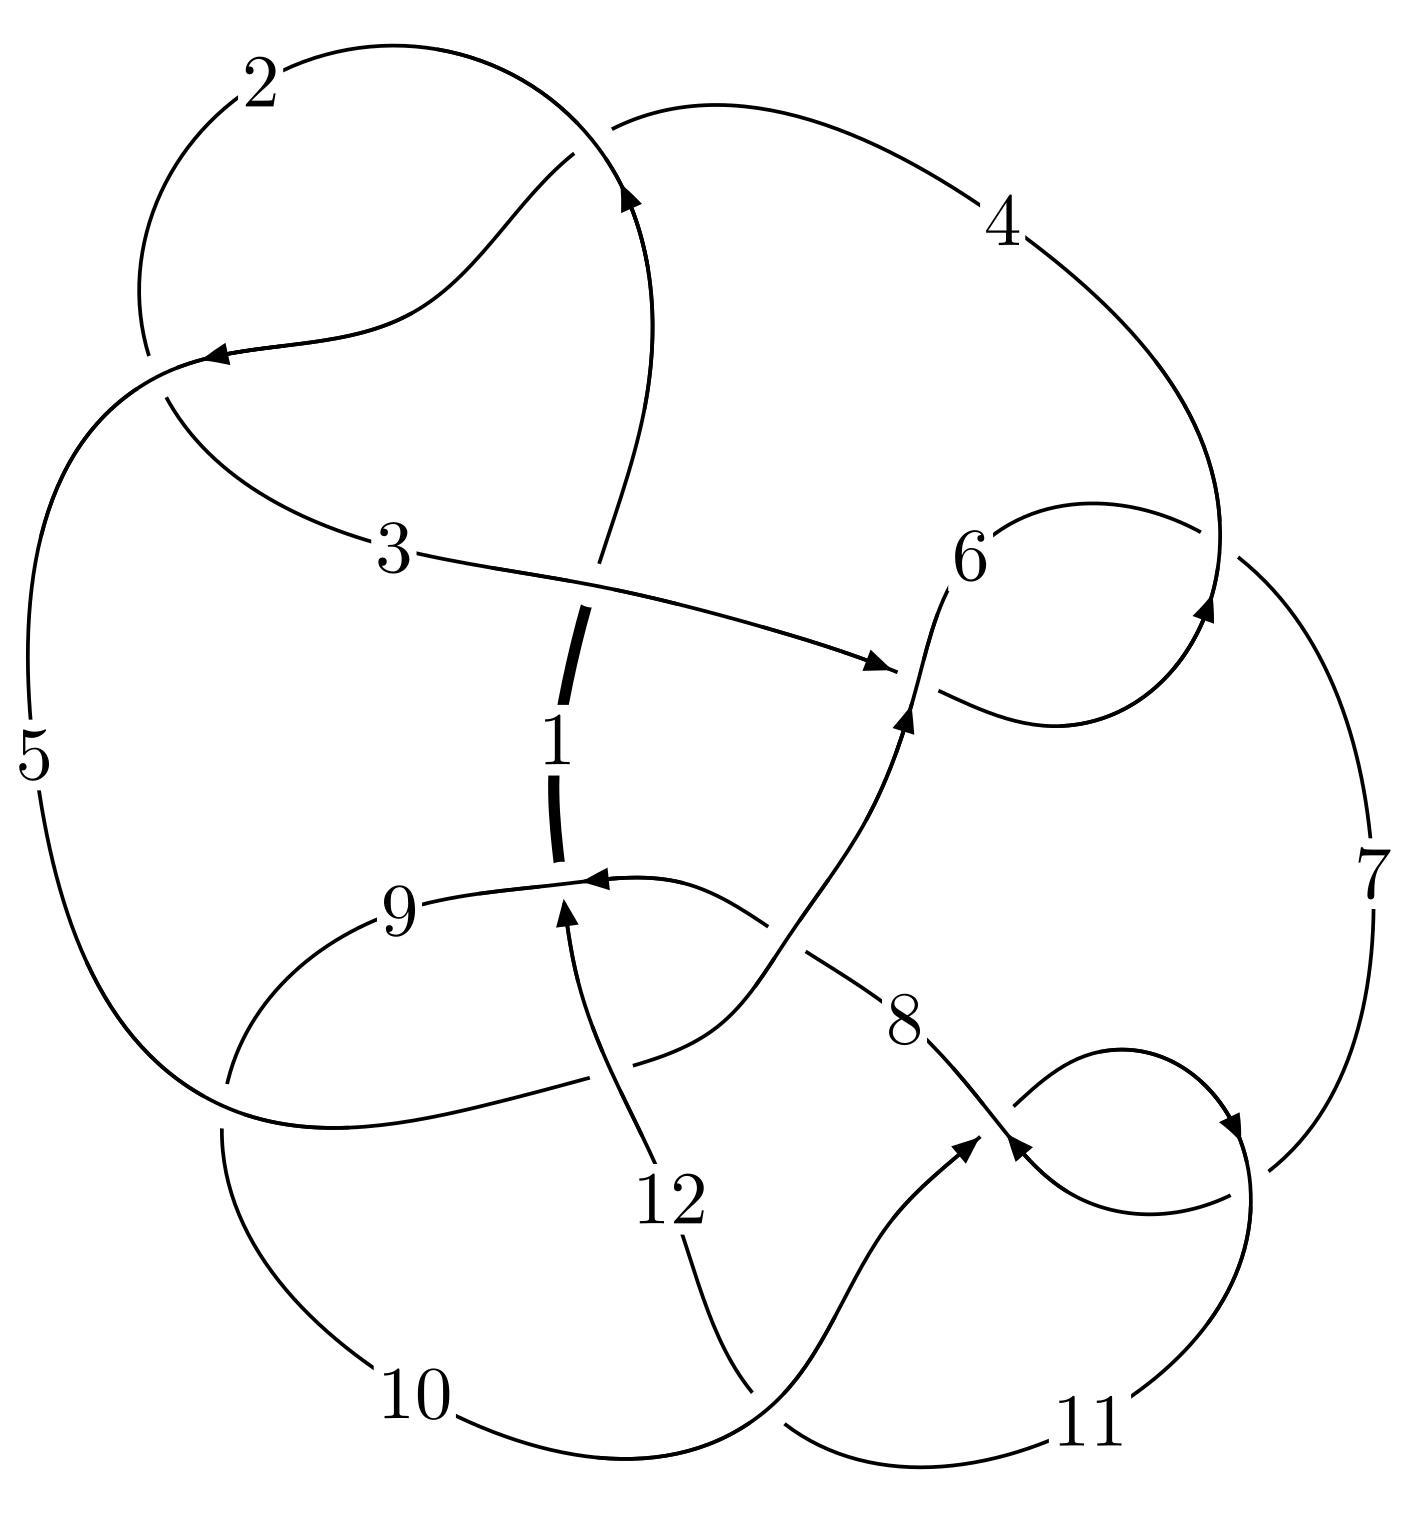
\includegraphics[width=112pt]{../../../GIT/diagram.site/Diagrams/png/2213_12n_0124.png}\\
\ \ \ A knot diagram\footnotemark}&
\allowdisplaybreaks
\textbf{Linearized knot diagam} \\
\cline{2-2}
 &
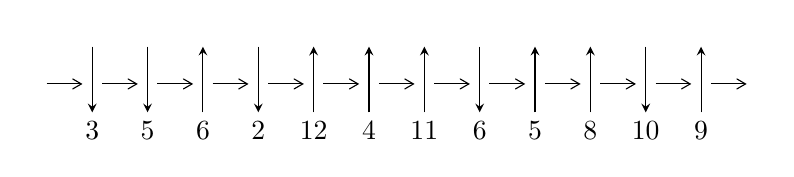
\begin{tikzpicture}[x=20pt, y=17pt]
	% nodes
	\node (C0) at (0, 0) {};
	\node (C1) at (1, 0) {};
	\node (C1U) at (1, +1) {};
	\node (C1D) at (1, -1) {3};

	\node (C2) at (2, 0) {};
	\node (C2U) at (2, +1) {};
	\node (C2D) at (2, -1) {5};

	\node (C3) at (3, 0) {};
	\node (C3U) at (3, +1) {};
	\node (C3D) at (3, -1) {6};

	\node (C4) at (4, 0) {};
	\node (C4U) at (4, +1) {};
	\node (C4D) at (4, -1) {2};

	\node (C5) at (5, 0) {};
	\node (C5U) at (5, +1) {};
	\node (C5D) at (5, -1) {12};

	\node (C6) at (6, 0) {};
	\node (C6U) at (6, +1) {};
	\node (C6D) at (6, -1) {4};

	\node (C7) at (7, 0) {};
	\node (C7U) at (7, +1) {};
	\node (C7D) at (7, -1) {11};

	\node (C8) at (8, 0) {};
	\node (C8U) at (8, +1) {};
	\node (C8D) at (8, -1) {6};

	\node (C9) at (9, 0) {};
	\node (C9U) at (9, +1) {};
	\node (C9D) at (9, -1) {5};

	\node (C10) at (10, 0) {};
	\node (C10U) at (10, +1) {};
	\node (C10D) at (10, -1) {8};

	\node (C11) at (11, 0) {};
	\node (C11U) at (11, +1) {};
	\node (C11D) at (11, -1) {10};

	\node (C12) at (12, 0) {};
	\node (C12U) at (12, +1) {};
	\node (C12D) at (12, -1) {9};
	\node (C13) at (13, 0) {};

	% arrows
	\draw[->,>={angle 60}]
	(C0) edge (C1) (C1) edge (C2) (C2) edge (C3) (C3) edge (C4) (C4) edge (C5) (C5) edge (C6) (C6) edge (C7) (C7) edge (C8) (C8) edge (C9) (C9) edge (C10) (C10) edge (C11) (C11) edge (C12) (C12) edge (C13) ;	\draw[->,>=stealth]
	(C1U) edge (C1D) (C2U) edge (C2D) (C3D) edge (C3U) (C4U) edge (C4D) (C5D) edge (C5U) (C6D) edge (C6U) (C7D) edge (C7U) (C8U) edge (C8D) (C9D) edge (C9U) (C10D) edge (C10U) (C11U) edge (C11D) (C12D) edge (C12U) ;
	\end{tikzpicture} \\
\hhline{~~} \\& 
\textbf{Solving Sequence} \\ \cline{2-2} 
 &
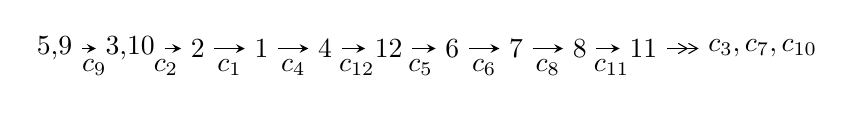
\begin{tikzpicture}[x=23pt, y=7pt]
	% node
	\node (A0) at (-1/8, 0) {5,9};
	\node (A1) at (17/16, 0) {3,10};
	\node (A2) at (17/8, 0) {2};
	\node (A3) at (25/8, 0) {1};
	\node (A4) at (33/8, 0) {4};
	\node (A5) at (41/8, 0) {12};
	\node (A6) at (49/8, 0) {6};
	\node (A7) at (57/8, 0) {7};
	\node (A8) at (65/8, 0) {8};
	\node (A9) at (73/8, 0) {11};
	\node (C1) at (1/2, -1) {$c_{9}$};
	\node (C2) at (13/8, -1) {$c_{2}$};
	\node (C3) at (21/8, -1) {$c_{1}$};
	\node (C4) at (29/8, -1) {$c_{4}$};
	\node (C5) at (37/8, -1) {$c_{12}$};
	\node (C6) at (45/8, -1) {$c_{5}$};
	\node (C7) at (53/8, -1) {$c_{6}$};
	\node (C8) at (61/8, -1) {$c_{8}$};
	\node (C9) at (69/8, -1) {$c_{11}$};
	\node (A10) at (11, 0) {$c_{3},c_{7},c_{10}$};

	% edge
	\draw[->,>=stealth]	
	(A0) edge (A1) (A1) edge (A2) (A2) edge (A3) (A3) edge (A4) (A4) edge (A5) (A5) edge (A6) (A6) edge (A7) (A7) edge (A8) (A8) edge (A9) ;
	\draw[->>,>={angle 60}]	
	(A9) edge (A10);
\end{tikzpicture} \\ 

\end{tabular} \\

\footnotetext{
The image of knot diagram is generated by the software ``\textbf{Draw programme}" developed by Andrew Bartholomew(\url{http://www.layer8.co.uk/maths/draw/index.htm\#Running-draw}), where we modified some parts for our purpose(\url{https://github.com/CATsTAILs/LinksPainter}).
}\phantom \\ \newline 
\centering \textbf{Ideals for irreducible components\footnotemark of $X_{\text{par}}$} 
 
\begin{align*}
I^u_{1}&=\langle 
-2.08067\times10^{71} u^{23}+5.26175\times10^{71} u^{22}+\cdots+2.02018\times10^{76} b-3.78380\times10^{76},\\
\phantom{I^u_{1}}&\phantom{= \langle  }9.08915\times10^{75} u^{23}+2.34052\times10^{76} u^{22}+\cdots+3.92744\times10^{80} a-1.11660\times10^{81},\\
\phantom{I^u_{1}}&\phantom{= \langle  }u^{24}- u^{23}+\cdots+74162 u-19441\rangle \\
I^u_{2}&=\langle 
-967 u^{11}-301 u^{10}+\cdots+263 b-1376,\;-1506 u^{11}-552 u^{10}+\cdots+263 a-2561,\\
\phantom{I^u_{2}}&\phantom{= \langle  }u^{12}+u^{11}- u^{10}-6 u^9-5 u^8+u^7+5 u^6+9 u^5+11 u^4+7 u^3+4 u^2+3 u+1\rangle \\
I^u_{3}&=\langle 
u^7-3 u^5- u^4+4 u^3+2 u^2+b- u-2,\;- u^8- u^7+2 u^6+3 u^5- u^4-3 u^3-2 u^2+a+1,\\
\phantom{I^u_{3}}&\phantom{= \langle  }u^9+u^8-2 u^7-3 u^6+u^5+3 u^4+2 u^3- u-1\rangle \\
\\
\end{align*}
\raggedright * 3 irreducible components of $\dim_{\mathbb{C}}=0$, with total 45 representations.\\
\footnotetext{All coefficients of polynomials are rational numbers. But the coefficients are sometimes approximated in decimal forms when there is not enough margin.}
\newpage
\renewcommand{\arraystretch}{1}
\centering \section*{I. $I^u_{1}= \langle -2.08\times10^{71} u^{23}+5.26\times10^{71} u^{22}+\cdots+2.02\times10^{76} b-3.78\times10^{76},\;9.09\times10^{75} u^{23}+2.34\times10^{76} u^{22}+\cdots+3.93\times10^{80} a-1.12\times10^{81},\;u^{24}- u^{23}+\cdots+74162 u-19441 \rangle$}
\flushleft \textbf{(i) Arc colorings}\\
\begin{tabular}{m{7pt} m{180pt} m{7pt} m{180pt} }
\flushright $a_{5}=$&$\begin{pmatrix}0\\u\end{pmatrix}$ \\
\flushright $a_{9}=$&$\begin{pmatrix}1\\0\end{pmatrix}$ \\
\flushright $a_{3}=$&$\begin{pmatrix}-0.0000231427 u^{23}-0.0000595940 u^{22}+\cdots-5.73288 u+2.84308\\0.0000102994 u^{23}-0.0000260459 u^{22}+\cdots-3.68024 u+1.87300\end{pmatrix}$ \\
\flushright $a_{10}=$&$\begin{pmatrix}1\\- u^2\end{pmatrix}$ \\
\flushright $a_{2}=$&$\begin{pmatrix}-0.0000231427 u^{23}-0.0000595940 u^{22}+\cdots-5.73288 u+2.84308\\0.0000614617 u^{23}-0.0000856774 u^{22}+\cdots-9.36624 u+3.48148\end{pmatrix}$ \\
\flushright $a_{1}=$&$\begin{pmatrix}-0.000169431 u^{23}+0.0000106683 u^{22}+\cdots+8.83572 u-1.35661\\0.0000252125 u^{23}-0.0000460045 u^{22}+\cdots-4.17125 u+1.93008\end{pmatrix}$ \\
\flushright $a_{4}=$&$\begin{pmatrix}0.0000635308 u^{23}-0.0000949036 u^{22}+\cdots-11.6803 u+4.35857\\0.0000714189 u^{23}-0.0000219756 u^{22}+\cdots-6.67895 u+2.17463\end{pmatrix}$ \\
\flushright $a_{12}=$&$\begin{pmatrix}-0.000194644 u^{23}+0.0000566729 u^{22}+\cdots+13.0070 u-3.28669\\0.0000252125 u^{23}-0.0000460045 u^{22}+\cdots-4.17125 u+1.93008\end{pmatrix}$ \\
\flushright $a_{6}=$&$\begin{pmatrix}0.0000728869 u^{23}+0.0000468189 u^{22}+\cdots-0.0880205 u+0.0552699\\-0.000132323 u^{23}+0.0000178400 u^{22}+\cdots+9.20508 u-2.72140\end{pmatrix}$ \\
\flushright $a_{7}=$&$\begin{pmatrix}0.000289264 u^{23}-0.0000276884 u^{22}+\cdots-16.0214 u+4.12000\\-0.000164735 u^{23}+0.0000153960 u^{22}+\cdots+10.2669 u-3.73292\end{pmatrix}$ \\
\flushright $a_{8}=$&$\begin{pmatrix}-0.000179309 u^{23}+0.0000323990 u^{22}+\cdots+9.44236 u-2.06987\\0.0000244553 u^{23}-0.0000672943 u^{22}+\cdots-5.21820 u+1.94011\end{pmatrix}$ \\
\flushright $a_{11}=$&$\begin{pmatrix}-0.000262366 u^{23}+0.0000264100 u^{22}+\cdots+15.2839 u-4.03891\\0.000137186 u^{23}-0.0000456660 u^{22}+\cdots-10.1214 u+3.83499\end{pmatrix}$\\&\end{tabular}
\flushleft \textbf{(ii) Obstruction class $= -1$}\\~\\
\flushleft \textbf{(iii) Cusp Shapes $= -0.0000679815 u^{23}-0.000171030 u^{22}+\cdots-11.2729 u+1.52274$}\\~\\
\newpage\renewcommand{\arraystretch}{1}
\flushleft \textbf{(iv) u-Polynomials at the component}\newline \\
\begin{tabular}{m{50pt}|m{274pt}}
Crossings & \hspace{64pt}u-Polynomials at each crossing \\
\hline $$\begin{aligned}c_{1}\end{aligned}$$&$\begin{aligned}
&u^{24}+24 u^{23}+\cdots-179 u+1
\end{aligned}$\\
\hline $$\begin{aligned}c_{2},c_{4}\end{aligned}$$&$\begin{aligned}
&u^{24}-12 u^{23}+\cdots+17 u-1
\end{aligned}$\\
\hline $$\begin{aligned}c_{3},c_{6}\end{aligned}$$&$\begin{aligned}
&u^{24}+u^{23}+\cdots-2560 u+512
\end{aligned}$\\
\hline $$\begin{aligned}c_{5}\end{aligned}$$&$\begin{aligned}
&u^{24}+4 u^{23}+\cdots-3 u-1
\end{aligned}$\\
\hline $$\begin{aligned}c_{7},c_{10}\end{aligned}$$&$\begin{aligned}
&u^{24}+8 u^{23}+\cdots+7 u+1
\end{aligned}$\\
\hline $$\begin{aligned}c_{8}\end{aligned}$$&$\begin{aligned}
&u^{24}-5 u^{23}+\cdots-389242 u+249139
\end{aligned}$\\
\hline $$\begin{aligned}c_{9}\end{aligned}$$&$\begin{aligned}
&u^{24}+u^{23}+\cdots-74162 u-19441
\end{aligned}$\\
\hline $$\begin{aligned}c_{11}\end{aligned}$$&$\begin{aligned}
&u^{24}+20 u^{22}+\cdots+19 u+1
\end{aligned}$\\
\hline $$\begin{aligned}c_{12}\end{aligned}$$&$\begin{aligned}
&u^{24}+2 u^{23}+\cdots+28672 u+4096
\end{aligned}$\\
\hline
\end{tabular}\\~\\
\newpage\renewcommand{\arraystretch}{1}
\flushleft \textbf{(v) Riley Polynomials at the component}\newline \\
\begin{tabular}{m{50pt}|m{274pt}}
Crossings & \hspace{64pt}Riley Polynomials at each crossing \\
\hline $$\begin{aligned}c_{1}\end{aligned}$$&$\begin{aligned}
&y^{24}+204 y^{23}+\cdots-2901 y+1
\end{aligned}$\\
\hline $$\begin{aligned}c_{2},c_{4}\end{aligned}$$&$\begin{aligned}
&y^{24}-24 y^{23}+\cdots+179 y+1
\end{aligned}$\\
\hline $$\begin{aligned}c_{3},c_{6}\end{aligned}$$&$\begin{aligned}
&y^{24}-63 y^{23}+\cdots-3932160 y+262144
\end{aligned}$\\
\hline $$\begin{aligned}c_{5}\end{aligned}$$&$\begin{aligned}
&y^{24}+26 y^{22}+\cdots- y+1
\end{aligned}$\\
\hline $$\begin{aligned}c_{7},c_{10}\end{aligned}$$&$\begin{aligned}
&y^{24}+20 y^{22}+\cdots+19 y+1
\end{aligned}$\\
\hline $$\begin{aligned}c_{8}\end{aligned}$$&$\begin{aligned}
&y^{24}+111 y^{23}+\cdots-469614992544 y+62070241321
\end{aligned}$\\
\hline $$\begin{aligned}c_{9}\end{aligned}$$&$\begin{aligned}
&y^{24}-61 y^{23}+\cdots-296113128 y+377952481
\end{aligned}$\\
\hline $$\begin{aligned}c_{11}\end{aligned}$$&$\begin{aligned}
&y^{24}+40 y^{23}+\cdots+2151 y+1
\end{aligned}$\\
\hline $$\begin{aligned}c_{12}\end{aligned}$$&$\begin{aligned}
&y^{24}-90 y^{23}+\cdots+67108864 y+16777216
\end{aligned}$\\
\hline
\end{tabular}\\~\\
\newpage\flushleft \textbf{(vi) Complex Volumes and Cusp Shapes}
$$\begin{array}{c|c|c}  
\text{Solutions to }I^u_{1}& \I (\text{vol} + \sqrt{-1}CS) & \text{Cusp shape}\\
 \hline 
\begin{aligned}
u &= \phantom{-}1.001080 + 0.138094 I \\
a &= -1.318540 - 0.227339 I \\
b &= \phantom{-}0.349925 + 0.133105 I\end{aligned}
 & \phantom{-}1.03909 - 7.66938 I & \phantom{-}3.58752 + 6.84907 I \\ \hline\begin{aligned}
u &= \phantom{-}1.001080 - 0.138094 I \\
a &= -1.318540 + 0.227339 I \\
b &= \phantom{-}0.349925 - 0.133105 I\end{aligned}
 & \phantom{-}1.03909 + 7.66938 I & \phantom{-}3.58752 - 6.84907 I \\ \hline\begin{aligned}
u &= -0.824749 + 0.684019 I \\
a &= \phantom{-}0.924018 + 0.059095 I \\
b &= -0.397533 + 0.099117 I\end{aligned}
 & \phantom{-}2.67249 - 0.06243 I & \phantom{-}6.49122 - 0.13400 I \\ \hline\begin{aligned}
u &= -0.824749 - 0.684019 I \\
a &= \phantom{-}0.924018 - 0.059095 I \\
b &= -0.397533 - 0.099117 I\end{aligned}
 & \phantom{-}2.67249 + 0.06243 I & \phantom{-}6.49122 + 0.13400 I \\ \hline\begin{aligned}
u &= \phantom{-}0.316783 + 0.857620 I \\
a &= \phantom{-}0.0626489 + 0.0577118 I \\
b &= -0.019035 + 0.639183 I\end{aligned}
 & \phantom{-}0.59509 - 2.36713 I & \phantom{-}1.40991 + 3.67925 I \\ \hline\begin{aligned}
u &= \phantom{-}0.316783 - 0.857620 I \\
a &= \phantom{-}0.0626489 - 0.0577118 I \\
b &= -0.019035 - 0.639183 I\end{aligned}
 & \phantom{-}0.59509 + 2.36713 I & \phantom{-}1.40991 - 3.67925 I \\ \hline\begin{aligned}
u &= \phantom{-}0.688053 + 0.891806 I \\
a &= \phantom{-}0.334387 + 0.540212 I \\
b &= \phantom{-}0.461704 + 0.711317 I\end{aligned}
 & -1.87950 + 2.72151 I & \phantom{-}1.13774 - 4.25269 I \\ \hline\begin{aligned}
u &= \phantom{-}0.688053 - 0.891806 I \\
a &= \phantom{-}0.334387 - 0.540212 I \\
b &= \phantom{-}0.461704 - 0.711317 I\end{aligned}
 & -1.87950 - 2.72151 I & \phantom{-}1.13774 + 4.25269 I \\ \hline\begin{aligned}
u &= -0.787218\phantom{ +0.000000I} \\
a &= \phantom{-}0.180911\phantom{ +0.000000I} \\
b &= -0.560374\phantom{ +0.000000I}\end{aligned}
 & \phantom{-}1.02845\phantom{ +0.000000I} & \phantom{-}10.2860\phantom{ +0.000000I} \\ \hline\begin{aligned}
u &= \phantom{-}0.834451 + 0.915879 I \\
a &= \phantom{-}0.352399 - 0.454795 I \\
b &= \phantom{-}2.73766 + 0.36092 I\end{aligned}
 & -1.38798 + 2.82419 I & \phantom{-}0.59813 - 2.55909 I\\
 \hline 
 \end{array}$$\newpage$$\begin{array}{c|c|c}  
\text{Solutions to }I^u_{1}& \I (\text{vol} + \sqrt{-1}CS) & \text{Cusp shape}\\
 \hline 
\begin{aligned}
u &= \phantom{-}0.834451 - 0.915879 I \\
a &= \phantom{-}0.352399 + 0.454795 I \\
b &= \phantom{-}2.73766 - 0.36092 I\end{aligned}
 & -1.38798 - 2.82419 I & \phantom{-}0.59813 + 2.55909 I \\ \hline\begin{aligned}
u &= \phantom{-}0.314005 + 0.468028 I \\
a &= \phantom{-}0.35394 - 1.75927 I \\
b &= \phantom{-}0.255305 - 0.819135 I\end{aligned}
 & -1.83062 + 1.07717 I & -2.53581 - 1.58170 I \\ \hline\begin{aligned}
u &= \phantom{-}0.314005 - 0.468028 I \\
a &= \phantom{-}0.35394 + 1.75927 I \\
b &= \phantom{-}0.255305 + 0.819135 I\end{aligned}
 & -1.83062 - 1.07717 I & -2.53581 + 1.58170 I \\ \hline\begin{aligned}
u &= \phantom{-}1.51494\phantom{ +0.000000I} \\
a &= \phantom{-}1.23042\phantom{ +0.000000I} \\
b &= \phantom{-}0.320247\phantom{ +0.000000I}\end{aligned}
 & \phantom{-}0.756608\phantom{ +0.000000I} & \phantom{-}8.01810\phantom{ +0.000000I} \\ \hline\begin{aligned}
u &= -1.50875 + 0.34715 I \\
a &= -0.824302 - 0.166530 I \\
b &= \phantom{-}2.22948 - 1.08324 I\end{aligned}
 & -2.60567 + 1.37963 I & -1.96914 - 4.05392 I \\ \hline\begin{aligned}
u &= -1.50875 - 0.34715 I \\
a &= -0.824302 + 0.166530 I \\
b &= \phantom{-}2.22948 + 1.08324 I\end{aligned}
 & -2.60567 - 1.37963 I & -1.96914 + 4.05392 I \\ \hline\begin{aligned}
u &= \phantom{-}1.93298 + 1.06740 I \\
a &= -0.453811 + 0.766464 I \\
b &= \phantom{-}0.08195 + 1.96919 I\end{aligned}
 & \phantom{-}18.8685 + 6.6483 I & \phantom{-}2.16489 - 2.21174 I \\ \hline\begin{aligned}
u &= \phantom{-}1.93298 - 1.06740 I \\
a &= -0.453811 - 0.766464 I \\
b &= \phantom{-}0.08195 - 1.96919 I\end{aligned}
 & \phantom{-}18.8685 - 6.6483 I & \phantom{-}2.16489 + 2.21174 I \\ \hline\begin{aligned}
u &= -2.70737 + 1.34412 I \\
a &= \phantom{-}0.343417 + 0.565612 I \\
b &= -0.11926 + 2.26369 I\end{aligned}
 & \phantom{-}18.7357 - 14.2573 I & \phantom{-0.000000 -}0. + 5.97304 I \\ \hline\begin{aligned}
u &= -2.70737 - 1.34412 I \\
a &= \phantom{-}0.343417 - 0.565612 I \\
b &= -0.11926 - 2.26369 I\end{aligned}
 & \phantom{-}18.7357 + 14.2573 I & \phantom{-0.000000 } 0. - 5.97304 I\\
 \hline 
 \end{array}$$\newpage$$\begin{array}{c|c|c}  
\text{Solutions to }I^u_{1}& \I (\text{vol} + \sqrt{-1}CS) & \text{Cusp shape}\\
 \hline 
\begin{aligned}
u &= \phantom{-}3.59990 + 1.47900 I \\
a &= -0.314174 + 0.597363 I \\
b &= \phantom{-}0.16845 + 2.06886 I\end{aligned}
 & -18.5925 + 5.6388 I & \phantom{-0.000000 } 0 \\ \hline\begin{aligned}
u &= \phantom{-}3.59990 - 1.47900 I \\
a &= -0.314174 - 0.597363 I \\
b &= \phantom{-}0.16845 - 2.06886 I\end{aligned}
 & -18.5925 - 5.6388 I & \phantom{-0.000000 } 0 \\ \hline\begin{aligned}
u &= -3.51025 + 2.07425 I \\
a &= \phantom{-}0.212826 + 0.620986 I \\
b &= -0.12859 + 2.14471 I\end{aligned}
 & -18.9745 + 1.9748 I & \phantom{-0.000000 } 0 \\ \hline\begin{aligned}
u &= -3.51025 - 2.07425 I \\
a &= \phantom{-}0.212826 - 0.620986 I \\
b &= -0.12859 - 2.14471 I\end{aligned}
 & -18.9745 - 1.9748 I & \phantom{-0.000000 } 0\\
 \hline 
 \end{array}$$\newpage\newpage\renewcommand{\arraystretch}{1}
\centering \section*{II. $I^u_{2}= \langle -967 u^{11}-301 u^{10}+\cdots+263 b-1376,\;-1506 u^{11}-552 u^{10}+\cdots+263 a-2561,\;u^{12}+u^{11}+\cdots+3 u+1 \rangle$}
\flushleft \textbf{(i) Arc colorings}\\
\begin{tabular}{m{7pt} m{180pt} m{7pt} m{180pt} }
\flushright $a_{5}=$&$\begin{pmatrix}0\\u\end{pmatrix}$ \\
\flushright $a_{9}=$&$\begin{pmatrix}1\\0\end{pmatrix}$ \\
\flushright $a_{3}=$&$\begin{pmatrix}5.72624 u^{11}+2.09886 u^{10}+\cdots+14.5894 u+9.73764\\3.67681 u^{11}+1.14449 u^{10}+\cdots+9.01521 u+5.23194\end{pmatrix}$ \\
\flushright $a_{10}=$&$\begin{pmatrix}1\\- u^2\end{pmatrix}$ \\
\flushright $a_{2}=$&$\begin{pmatrix}5.72624 u^{11}+2.09886 u^{10}+\cdots+14.5894 u+9.73764\\1.23954 u^{11}+0.163498 u^{10}+\cdots+3.85932 u+1.60456\end{pmatrix}$ \\
\flushright $a_{1}=$&$\begin{pmatrix}-7.99620 u^{11}-1.69582 u^{10}+\cdots-17.4943 u-11.0380\\0\end{pmatrix}$ \\
\flushright $a_{4}=$&$\begin{pmatrix}-10.4525 u^{11}-3.19772 u^{10}+\cdots-25.1787 u-16.4753\\1.81369 u^{11}+1.09506 u^{10}+\cdots+4.22053 u+2.86312\end{pmatrix}$ \\
\flushright $a_{12}=$&$\begin{pmatrix}-7.99620 u^{11}-1.69582 u^{10}+\cdots-17.4943 u-11.0380\\0\end{pmatrix}$ \\
\flushright $a_{6}=$&$\begin{pmatrix}16.0380 u^{11}+5.04183 u^{10}+\cdots+39.0570 u+25.6198\\u\end{pmatrix}$ \\
\flushright $a_{7}=$&$\begin{pmatrix}7.99620 u^{11}+1.69582 u^{10}+\cdots+17.4943 u+11.0380\\0\end{pmatrix}$ \\
\flushright $a_{8}=$&$\begin{pmatrix}10.9962 u^{11}+3.69582 u^{10}+\cdots+22.4943 u+17.0380\\- u^2\end{pmatrix}$ \\
\flushright $a_{11}=$&$\begin{pmatrix}-12.2662 u^{11}-3.29278 u^{10}+\cdots-28.3992 u-17.3384\\1.83270 u^{11}+0.615970 u^{10}+\cdots+3.74905 u+2.67300\end{pmatrix}$\\&\end{tabular}
\flushleft \textbf{(ii) Obstruction class $= 1$}\\~\\
\flushleft \textbf{(iii) Cusp Shapes $= \frac{9447}{263} u^{11}+\frac{3054}{263} u^{10}-\frac{11456}{263} u^9-\frac{49096}{263} u^8-\frac{14483}{263} u^7+\frac{18808}{263} u^6+\frac{35545}{263} u^5+\frac{63461}{263} u^4+\frac{61950}{263} u^3+\frac{23143}{263} u^2+\frac{19562}{263} u+\frac{13360}{263}$}\\~\\
\newpage\renewcommand{\arraystretch}{1}
\flushleft \textbf{(iv) u-Polynomials at the component}\newline \\
\begin{tabular}{m{50pt}|m{274pt}}
Crossings & \hspace{64pt}u-Polynomials at each crossing \\
\hline $$\begin{aligned}c_{1},c_{5}\end{aligned}$$&$\begin{aligned}
&(u^6-3 u^5+5 u^4-4 u^3+2 u^2- u+1)^2
\end{aligned}$\\
\hline $$\begin{aligned}c_{2},c_{6}\end{aligned}$$&$\begin{aligned}
&(u^6+u^5- u^4-2 u^3+u+1)^2
\end{aligned}$\\
\hline $$\begin{aligned}c_{3},c_{4}\end{aligned}$$&$\begin{aligned}
&(u^6- u^5- u^4+2 u^3- u+1)^2
\end{aligned}$\\
\hline $$\begin{aligned}c_{7},c_{11}\end{aligned}$$&$\begin{aligned}
&(u^2+u+1)^6
\end{aligned}$\\
\hline $$\begin{aligned}c_{8},c_{9}\end{aligned}$$&$\begin{aligned}
&u^{12}+u^{11}+\cdots+3 u+1
\end{aligned}$\\
\hline $$\begin{aligned}c_{10}\end{aligned}$$&$\begin{aligned}
&(u^2- u+1)^6
\end{aligned}$\\
\hline $$\begin{aligned}c_{12}\end{aligned}$$&$\begin{aligned}
&u^{12}
\end{aligned}$\\
\hline
\end{tabular}\\~\\
\newpage\renewcommand{\arraystretch}{1}
\flushleft \textbf{(v) Riley Polynomials at the component}\newline \\
\begin{tabular}{m{50pt}|m{274pt}}
Crossings & \hspace{64pt}Riley Polynomials at each crossing \\
\hline $$\begin{aligned}c_{1},c_{5}\end{aligned}$$&$\begin{aligned}
&(y^6+y^5+5 y^4+6 y^2+3 y+1)^2
\end{aligned}$\\
\hline $$\begin{aligned}c_{2},c_{3},c_{4}\\c_{6}\end{aligned}$$&$\begin{aligned}
&(y^6-3 y^5+5 y^4-4 y^3+2 y^2- y+1)^2
\end{aligned}$\\
\hline $$\begin{aligned}c_{7},c_{10},c_{11}\end{aligned}$$&$\begin{aligned}
&(y^2+y+1)^6
\end{aligned}$\\
\hline $$\begin{aligned}c_{8},c_{9}\end{aligned}$$&$\begin{aligned}
&y^{12}-3 y^{11}+\cdots- y+1
\end{aligned}$\\
\hline $$\begin{aligned}c_{12}\end{aligned}$$&$\begin{aligned}
&y^{12}
\end{aligned}$\\
\hline
\end{tabular}\\~\\
\newpage\flushleft \textbf{(vi) Complex Volumes and Cusp Shapes}
$$\begin{array}{c|c|c}  
\text{Solutions to }I^u_{2}& \I (\text{vol} + \sqrt{-1}CS) & \text{Cusp shape}\\
 \hline 
\begin{aligned}
u &= -0.815127 + 0.417821 I \\
a &= \phantom{-}0.746988 - 0.432355 I \\
b &= -0.167948 - 0.496751 I\end{aligned}
 & \phantom{-}1.89061 + 1.10558 I & \phantom{-}3.63443 - 2.52768 I \\ \hline\begin{aligned}
u &= -0.815127 - 0.417821 I \\
a &= \phantom{-}0.746988 + 0.432355 I \\
b &= -0.167948 + 0.496751 I\end{aligned}
 & \phantom{-}1.89061 - 1.10558 I & \phantom{-}3.63443 + 2.52768 I \\ \hline\begin{aligned}
u &= \phantom{-}0.045720 + 0.914831 I \\
a &= -0.747924 + 0.430733 I \\
b &= \phantom{-}0.514173 - 0.102928 I\end{aligned}
 & \phantom{-}1.89061 + 2.95419 I & \phantom{-}6.39280 - 3.57892 I \\ \hline\begin{aligned}
u &= \phantom{-}0.045720 - 0.914831 I \\
a &= -0.747924 - 0.430733 I \\
b &= \phantom{-}0.514173 + 0.102928 I\end{aligned}
 & \phantom{-}1.89061 - 2.95419 I & \phantom{-}6.39280 + 3.57892 I \\ \hline\begin{aligned}
u &= \phantom{-}0.288082 + 0.618530 I \\
a &= \phantom{-}0.07779 + 1.77253 I \\
b &= -0.483138 + 0.481819 I\end{aligned}
 & \phantom{-0.000000 -}7.72290 I & -2.53591 - 7.46338 I \\ \hline\begin{aligned}
u &= \phantom{-}0.288082 - 0.618530 I \\
a &= \phantom{-}0.07779 - 1.77253 I \\
b &= -0.483138 - 0.481819 I\end{aligned}
 & \phantom{-0.000000 } -7.72290 I & -2.53591 + 7.46338 I \\ \hline\begin{aligned}
u &= -0.679704 + 0.059778 I \\
a &= \phantom{-}1.49615 + 0.95363 I \\
b &= -0.175699 + 0.659319 I\end{aligned}
 & \phantom{-0.000000 } -3.66314 I & \phantom{-}2.83009 + 6.37777 I \\ \hline\begin{aligned}
u &= -0.679704 - 0.059778 I \\
a &= \phantom{-}1.49615 - 0.95363 I \\
b &= -0.175699 - 0.659319 I\end{aligned}
 & \phantom{-0.000000 -}3.66314 I & \phantom{-}2.83009 - 6.37777 I \\ \hline\begin{aligned}
u &= -0.93136 + 1.30101 I \\
a &= -0.214408 - 0.616830 I \\
b &= -2.00856 - 1.94349 I\end{aligned}
 & -1.89061 - 2.95419 I & -7.91752 + 1.81989 I \\ \hline\begin{aligned}
u &= -0.93136 - 1.30101 I \\
a &= -0.214408 + 0.616830 I \\
b &= -2.00856 + 1.94349 I\end{aligned}
 & -1.89061 + 2.95419 I & -7.91752 - 1.81989 I\\
 \hline 
 \end{array}$$\newpage$$\begin{array}{c|c|c}  
\text{Solutions to }I^u_{2}& \I (\text{vol} + \sqrt{-1}CS) & \text{Cusp shape}\\
 \hline 
\begin{aligned}
u &= \phantom{-}1.59239 + 0.15607 I \\
a &= \phantom{-}0.641395 + 0.122732 I \\
b &= -0.67883 + 2.71121 I\end{aligned}
 & -1.89061 + 1.10558 I & \phantom{-}3.59610 - 6.57635 I \\ \hline\begin{aligned}
u &= \phantom{-}1.59239 - 0.15607 I \\
a &= \phantom{-}0.641395 - 0.122732 I \\
b &= -0.67883 - 2.71121 I\end{aligned}
 & -1.89061 - 1.10558 I & \phantom{-}3.59610 + 6.57635 I\\
 \hline 
 \end{array}$$\newpage\newpage\renewcommand{\arraystretch}{1}
\centering \section*{III. $I^u_{3}= \langle u^7-3 u^5- u^4+4 u^3+2 u^2+b- u-2,\;- u^8- u^7+\cdots+a+1,\;u^9+u^8-2 u^7-3 u^6+u^5+3 u^4+2 u^3- u-1 \rangle$}
\flushleft \textbf{(i) Arc colorings}\\
\begin{tabular}{m{7pt} m{180pt} m{7pt} m{180pt} }
\flushright $a_{5}=$&$\begin{pmatrix}0\\u\end{pmatrix}$ \\
\flushright $a_{9}=$&$\begin{pmatrix}1\\0\end{pmatrix}$ \\
\flushright $a_{3}=$&$\begin{pmatrix}u^8+u^7-2 u^6-3 u^5+u^4+3 u^3+2 u^2-1\\- u^7+3 u^5+u^4-4 u^3-2 u^2+u+2\end{pmatrix}$ \\
\flushright $a_{10}=$&$\begin{pmatrix}1\\- u^2\end{pmatrix}$ \\
\flushright $a_{2}=$&$\begin{pmatrix}u^8+u^7-2 u^6-3 u^5+u^4+3 u^3+2 u^2-1\\- u^7+3 u^5+u^4-4 u^3-2 u^2+2\end{pmatrix}$ \\
\flushright $a_{1}=$&$\begin{pmatrix}0\\- u\end{pmatrix}$ \\
\flushright $a_{4}=$&$\begin{pmatrix}u^8+u^7-2 u^6-3 u^5+u^4+3 u^3+2 u^2-1\\- u^7+3 u^5+u^4-4 u^3-2 u^2+u+2\end{pmatrix}$ \\
\flushright $a_{12}=$&$\begin{pmatrix}u\\- u\end{pmatrix}$ \\
\flushright $a_{6}=$&$\begin{pmatrix}u^3\\- u^3+u\end{pmatrix}$ \\
\flushright $a_{7}=$&$\begin{pmatrix}u^3\\- u^3+u\end{pmatrix}$ \\
\flushright $a_{8}=$&$\begin{pmatrix}u^6- u^4+1\\- u^6+2 u^4- u^2\end{pmatrix}$ \\
\flushright $a_{11}=$&$\begin{pmatrix}u^3\\- u^5+u^3- u\end{pmatrix}$\\&\end{tabular}
\flushleft \textbf{(ii) Obstruction class $= 1$}\\~\\
\flushleft \textbf{(iii) Cusp Shapes $= -5 u^8- u^7+7 u^6+6 u^5-6 u^4-7 u^3-5 u^2+7 u+1$}\\~\\
\newpage\renewcommand{\arraystretch}{1}
\flushleft \textbf{(iv) u-Polynomials at the component}\newline \\
\begin{tabular}{m{50pt}|m{274pt}}
Crossings & \hspace{64pt}u-Polynomials at each crossing \\
\hline $$\begin{aligned}c_{1},c_{2}\end{aligned}$$&$\begin{aligned}
&(u-1)^9
\end{aligned}$\\
\hline $$\begin{aligned}c_{3},c_{6}\end{aligned}$$&$\begin{aligned}
&u^9
\end{aligned}$\\
\hline $$\begin{aligned}c_{4}\end{aligned}$$&$\begin{aligned}
&(u+1)^9
\end{aligned}$\\
\hline $$\begin{aligned}c_{5}\end{aligned}$$&$\begin{aligned}
&u^9+5 u^8+12 u^7+15 u^6+9 u^5- u^4-4 u^3-2 u^2+u+1
\end{aligned}$\\
\hline $$\begin{aligned}c_{7}\end{aligned}$$&$\begin{aligned}
&u^9- u^8+2 u^7- u^6+3 u^5- u^4+2 u^3+u+1
\end{aligned}$\\
\hline $$\begin{aligned}c_{8},c_{11}\end{aligned}$$&$\begin{aligned}
&u^9+3 u^8+8 u^7+13 u^6+17 u^5+17 u^4+12 u^3+6 u^2+u-1
\end{aligned}$\\
\hline $$\begin{aligned}c_{9},c_{12}\end{aligned}$$&$\begin{aligned}
&u^9+u^8-2 u^7-3 u^6+u^5+3 u^4+2 u^3- u-1
\end{aligned}$\\
\hline $$\begin{aligned}c_{10}\end{aligned}$$&$\begin{aligned}
&u^9+u^8+2 u^7+u^6+3 u^5+u^4+2 u^3+u-1
\end{aligned}$\\
\hline
\end{tabular}\\~\\
\newpage\renewcommand{\arraystretch}{1}
\flushleft \textbf{(v) Riley Polynomials at the component}\newline \\
\begin{tabular}{m{50pt}|m{274pt}}
Crossings & \hspace{64pt}Riley Polynomials at each crossing \\
\hline $$\begin{aligned}c_{1},c_{2},c_{4}\end{aligned}$$&$\begin{aligned}
&(y-1)^9
\end{aligned}$\\
\hline $$\begin{aligned}c_{3},c_{6}\end{aligned}$$&$\begin{aligned}
&y^9
\end{aligned}$\\
\hline $$\begin{aligned}c_{5}\end{aligned}$$&$\begin{aligned}
&y^9- y^8+12 y^7-7 y^6+37 y^5+y^4-10 y^2+5 y-1
\end{aligned}$\\
\hline $$\begin{aligned}c_{7},c_{10}\end{aligned}$$&$\begin{aligned}
&y^9+3 y^8+8 y^7+13 y^6+17 y^5+17 y^4+12 y^3+6 y^2+y-1
\end{aligned}$\\
\hline $$\begin{aligned}c_{8},c_{11}\end{aligned}$$&$\begin{aligned}
&y^9+7 y^8+20 y^7+25 y^6+5 y^5-15 y^4+22 y^2+13 y-1
\end{aligned}$\\
\hline $$\begin{aligned}c_{9},c_{12}\end{aligned}$$&$\begin{aligned}
&y^9-5 y^8+12 y^7-15 y^6+9 y^5+y^4-4 y^3+2 y^2+y-1
\end{aligned}$\\
\hline
\end{tabular}\\~\\
\newpage\flushleft \textbf{(vi) Complex Volumes and Cusp Shapes}
$$\begin{array}{c|c|c}  
\text{Solutions to }I^u_{3}& \I (\text{vol} + \sqrt{-1}CS) & \text{Cusp shape}\\
 \hline 
\begin{aligned}
u &= -0.772920 + 0.510351 I \\
a &= -0.900982 - 0.594909 I \\
b &= \phantom{-}1.126210 - 0.643329 I\end{aligned}
 & -3.42837 - 2.09337 I & -4.41045 + 5.46639 I \\ \hline\begin{aligned}
u &= -0.772920 - 0.510351 I \\
a &= -0.900982 + 0.594909 I \\
b &= \phantom{-}1.126210 + 0.643329 I\end{aligned}
 & -3.42837 + 2.09337 I & -4.41045 - 5.46639 I \\ \hline\begin{aligned}
u &= \phantom{-}0.825933\phantom{ +0.000000I} \\
a &= \phantom{-}1.21075\phantom{ +0.000000I} \\
b &= \phantom{-}0.564116\phantom{ +0.000000I}\end{aligned}
 & -0.446489\phantom{ +0.000000I} & -0.182090\phantom{ +0.000000I} \\ \hline\begin{aligned}
u &= \phantom{-}1.173910 + 0.391555 I \\
a &= \phantom{-}0.766570 - 0.255687 I \\
b &= -0.466457 - 0.178345 I\end{aligned}
 & \phantom{-}2.72642 + 1.33617 I & \phantom{-}8.07941 - 3.55369 I \\ \hline\begin{aligned}
u &= \phantom{-}1.173910 - 0.391555 I \\
a &= \phantom{-}0.766570 + 0.255687 I \\
b &= -0.466457 + 0.178345 I\end{aligned}
 & \phantom{-}2.72642 - 1.33617 I & \phantom{-}8.07941 + 3.55369 I \\ \hline\begin{aligned}
u &= -0.141484 + 0.739668 I \\
a &= -0.249476 - 1.304240 I \\
b &= \phantom{-}1.50705 + 3.27928 I\end{aligned}
 & -1.02799 + 2.45442 I & -2.24638 + 6.63381 I \\ \hline\begin{aligned}
u &= -0.141484 - 0.739668 I \\
a &= -0.249476 + 1.304240 I \\
b &= \phantom{-}1.50705 - 3.27928 I\end{aligned}
 & -1.02799 - 2.45442 I & -2.24638 - 6.63381 I \\ \hline\begin{aligned}
u &= -1.172470 + 0.500383 I \\
a &= -0.721488 - 0.307914 I \\
b &= \phantom{-}0.551136 - 0.143741 I\end{aligned}
 & \phantom{-}1.95319 - 7.08493 I & \phantom{-}8.66846 + 5.33071 I \\ \hline\begin{aligned}
u &= -1.172470 - 0.500383 I \\
a &= -0.721488 + 0.307914 I \\
b &= \phantom{-}0.551136 + 0.143741 I\end{aligned}
 & \phantom{-}1.95319 + 7.08493 I & \phantom{-}8.66846 - 5.33071 I\\
 \hline 
 \end{array}$$\newpage
\newpage\renewcommand{\arraystretch}{1}
\centering \section*{ IV. u-Polynomials}
\begin{tabular}{m{50pt}|m{274pt}}
Crossings & \hspace{64pt}u-Polynomials at each crossing \\
\hline $$\begin{aligned}c_{1}\end{aligned}$$&$\begin{aligned}
&(u-1)^9(u^6-3 u^5+5 u^4-4 u^3+2 u^2- u+1)^2\\
&\cdot(u^{24}+24 u^{23}+\cdots-179 u+1)
\end{aligned}$\\
\hline $$\begin{aligned}c_{2}\end{aligned}$$&$\begin{aligned}
&((u-1)^9)(u^6+u^5+\cdots+u+1)^{2}(u^{24}-12 u^{23}+\cdots+17 u-1)
\end{aligned}$\\
\hline $$\begin{aligned}c_{3}\end{aligned}$$&$\begin{aligned}
&u^9(u^6- u^5+\cdots- u+1)^{2}(u^{24}+u^{23}+\cdots-2560 u+512)
\end{aligned}$\\
\hline $$\begin{aligned}c_{4}\end{aligned}$$&$\begin{aligned}
&((u+1)^9)(u^6- u^5+\cdots- u+1)^{2}(u^{24}-12 u^{23}+\cdots+17 u-1)
\end{aligned}$\\
\hline $$\begin{aligned}c_{5}\end{aligned}$$&$\begin{aligned}
&(u^6-3 u^5+5 u^4-4 u^3+2 u^2- u+1)^2\\
&\cdot(u^9+5 u^8+12 u^7+15 u^6+9 u^5- u^4-4 u^3-2 u^2+u+1)\\
&\cdot(u^{24}+4 u^{23}+\cdots-3 u-1)
\end{aligned}$\\
\hline $$\begin{aligned}c_{6}\end{aligned}$$&$\begin{aligned}
&u^9(u^6+u^5+\cdots+u+1)^{2}(u^{24}+u^{23}+\cdots-2560 u+512)
\end{aligned}$\\
\hline $$\begin{aligned}c_{7}\end{aligned}$$&$\begin{aligned}
&(u^2+u+1)^6(u^9- u^8+2 u^7- u^6+3 u^5- u^4+2 u^3+u+1)\\
&\cdot(u^{24}+8 u^{23}+\cdots+7 u+1)
\end{aligned}$\\
\hline $$\begin{aligned}c_{8}\end{aligned}$$&$\begin{aligned}
&(u^9+3 u^8+8 u^7+13 u^6+17 u^5+17 u^4+12 u^3+6 u^2+u-1)\\
&\cdot(u^{12}+u^{11}+\cdots+3 u+1)(u^{24}-5 u^{23}+\cdots-389242 u+249139)
\end{aligned}$\\
\hline $$\begin{aligned}c_{9}\end{aligned}$$&$\begin{aligned}
&(u^9+u^8+\cdots- u-1)(u^{12}+u^{11}+\cdots+3 u+1)\\
&\cdot(u^{24}+u^{23}+\cdots-74162 u-19441)
\end{aligned}$\\
\hline $$\begin{aligned}c_{10}\end{aligned}$$&$\begin{aligned}
&(u^2- u+1)^6(u^9+u^8+2 u^7+u^6+3 u^5+u^4+2 u^3+u-1)\\
&\cdot(u^{24}+8 u^{23}+\cdots+7 u+1)
\end{aligned}$\\
\hline $$\begin{aligned}c_{11}\end{aligned}$$&$\begin{aligned}
&(u^2+u+1)^6\\
&\cdot(u^9+3 u^8+8 u^7+13 u^6+17 u^5+17 u^4+12 u^3+6 u^2+u-1)\\
&\cdot(u^{24}+20 u^{22}+\cdots+19 u+1)
\end{aligned}$\\
\hline $$\begin{aligned}c_{12}\end{aligned}$$&$\begin{aligned}
&u^{12}(u^9+u^8-2 u^7-3 u^6+u^5+3 u^4+2 u^3- u-1)\\
&\cdot(u^{24}+2 u^{23}+\cdots+28672 u+4096)
\end{aligned}$\\
\hline
\end{tabular}\newpage\renewcommand{\arraystretch}{1}
\centering \section*{ V. Riley Polynomials}
\begin{tabular}{m{50pt}|m{274pt}}
Crossings & \hspace{64pt}Riley Polynomials at each crossing \\
\hline $$\begin{aligned}c_{1}\end{aligned}$$&$\begin{aligned}
&(y-1)^9(y^6+y^5+5 y^4+6 y^2+3 y+1)^2\\
&\cdot(y^{24}+204 y^{23}+\cdots-2901 y+1)
\end{aligned}$\\
\hline $$\begin{aligned}c_{2},c_{4}\end{aligned}$$&$\begin{aligned}
&(y-1)^9(y^6-3 y^5+5 y^4-4 y^3+2 y^2- y+1)^2\\
&\cdot(y^{24}-24 y^{23}+\cdots+179 y+1)
\end{aligned}$\\
\hline $$\begin{aligned}c_{3},c_{6}\end{aligned}$$&$\begin{aligned}
&y^9(y^6-3 y^5+5 y^4-4 y^3+2 y^2- y+1)^2\\
&\cdot(y^{24}-63 y^{23}+\cdots-3932160 y+262144)
\end{aligned}$\\
\hline $$\begin{aligned}c_{5}\end{aligned}$$&$\begin{aligned}
&(y^6+y^5+5 y^4+6 y^2+3 y+1)^2\\
&\cdot(y^9- y^8+12 y^7-7 y^6+37 y^5+y^4-10 y^2+5 y-1)\\
&\cdot(y^{24}+26 y^{22}+\cdots- y+1)
\end{aligned}$\\
\hline $$\begin{aligned}c_{7},c_{10}\end{aligned}$$&$\begin{aligned}
&(y^2+y+1)^6\\
&\cdot(y^9+3 y^8+8 y^7+13 y^6+17 y^5+17 y^4+12 y^3+6 y^2+y-1)\\
&\cdot(y^{24}+20 y^{22}+\cdots+19 y+1)
\end{aligned}$\\
\hline $$\begin{aligned}c_{8}\end{aligned}$$&$\begin{aligned}
&(y^9+7 y^8+20 y^7+25 y^6+5 y^5-15 y^4+22 y^2+13 y-1)\\
&\cdot(y^{12}-3 y^{11}+\cdots- y+1)\\
&\cdot(y^{24}+111 y^{23}+\cdots-469614992544 y+62070241321)
\end{aligned}$\\
\hline $$\begin{aligned}c_{9}\end{aligned}$$&$\begin{aligned}
&(y^9-5 y^8+12 y^7-15 y^6+9 y^5+y^4-4 y^3+2 y^2+y-1)\\
&\cdot(y^{12}-3 y^{11}+\cdots- y+1)\\
&\cdot(y^{24}-61 y^{23}+\cdots-296113128 y+377952481)
\end{aligned}$\\
\hline $$\begin{aligned}c_{11}\end{aligned}$$&$\begin{aligned}
&((y^2+y+1)^6)(y^9+7 y^8+\cdots+13 y-1)\\
&\cdot(y^{24}+40 y^{23}+\cdots+2151 y+1)
\end{aligned}$\\
\hline $$\begin{aligned}c_{12}\end{aligned}$$&$\begin{aligned}
&y^{12}(y^9-5 y^8+12 y^7-15 y^6+9 y^5+y^4-4 y^3+2 y^2+y-1)\\
&\cdot(y^{24}-90 y^{23}+\cdots+67108864 y+16777216)
\end{aligned}$\\
\hline
\end{tabular}
\vskip 2pc
\end{document}